\section{Auswertung} \label{sec:auswertung}

Hinweis: Die 44232 aufgenommenen Messpunkte sind in diesem Protokoll nicht enthalten.
Unter Vorbehalt sind sie jedoch \href{https://github.com/NicoWeio/AP/tree/master/V204_Waermeleitung}{online abrufbar}.

In diesem Abschnitt werden aus den Messdaten
mithilfe der statischen Methode
Temperaturverläufe visualisiert,
der Stab mit der besten Wärmeleitung bestimmt,
und Wärmeströme in den Stäben berechnet.
Mithilfe der dynamischen Methode wird die Wärmeleitfähigkeit von Messing (breit), Aluminium und Edelstahl berechnet.

\subsection{statische Methode}

\subsubsection{graphische Darstellung und Vergleich der Temperaturverläufe}

In \autoref{fig:statisch_alle} ist die zeitliche Entwicklung der Temperatur der vier Metallstäbe jeweils am fernen Thermoelement dargestellt.

\begin{figure}[H]
  \centering
  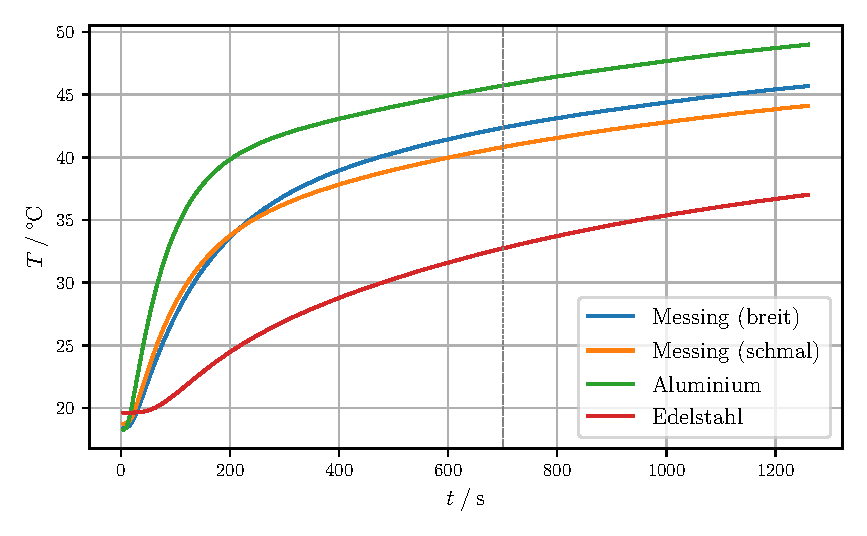
\includegraphics{build/plot_statisch_alle.pdf}
  \caption{Zeitliche Entwicklung der Temperatur (fern) der vier Metallstäbe.}
  \label{fig:statisch_alle}
\end{figure}

Die Temperaturverläufe der beiden Messingstäbe sind bis $\SI{300}{\second}$ nahezu identisch,
danach kommt der breite Messingstab jedoch auf eine konstant höhere Temperatur.
% Schuss ins Dunkle…
Eine mögliche Erklärung ist,
dass bei Vergrößerung des Stabs dessen Volumen schneller als die Oberfläche anwächst,
sodass weniger Wärme pro Volumeneinheit an der Oberfläche dissipieren kann.

Die Temperaturverläufe des Aluminium- und Edelstahlstabs
unterscheiden sich hingegen deutlich.
Die Temperatur des Aluminiumstabs steigt anfangs stark an und flacht nach und nach ab,
während die Temperatur des Edelstahls langsam, aber eher kontinuierlich zunimmt.
Diese Beobachtungen decken sich mit den in \autoref{sec:auswertung_dynamisch} berechneten Wärmeleitfähigkeiten.


\subsubsection{Bestimmung des Stabs mit der besten Wärmeleitung}

\begin{table}[H]
  \centering
  \caption{Temperaturen der fernen Thermoelemente nach $\SI{700}{\second}$.}
  \label{tab:temps_at_700}
  \begin{tabular}{l c}
  \toprule
  Material &
  $T \mathbin{/} \si{\celsius}$ \\
  \midrule
  \textbf{T1} (Messing, breit)  & \num{42.40} \\
  \textbf{T4} (Messing, schmal) & \num{40.85} \\
  \textbf{T5} (Aluminium)       & \num{45.75} \\
  \textbf{T8} (Edelstahl)       & \num{32.78} \\
  \bottomrule
  \end{tabular}
\end{table}

Nach $\SI{700}{\second}$ hat \textbf{T5} mit $\SI{45.75}{\celsius}$ die höchste Temperatur,
wie \autoref{tab:temps_at_700} zu entnehmen ist.
Dementsprechend hat Aluminium die beste Wärmeleitfähigkeit.
Auch diese Feststellung deckt sich mit den \hyperref[tab:daten_vorbereitung]{Literaturwerten}.


\subsubsection{Berechnung von Wärmeströmen}

Mithilfe der Gleichungen \eqref{eqn:waermemenge_pro_zeit} und \eqref{eqn:waermestromdichte}
sowie der in \autoref{tab:daten_vorbereitung} dargestellten Literaturwerte für die Wärmeleitfähigkeit
kann nun der Wärmestrom in den Stäben berechnet werden.
$\frac{\partial T}{\partial x}$ ist hier die Temperaturdifferenz der nahen und fernen Thermoelemente geteilt durch deren Abstand $\SI{3}{\centi\meter}$.
Der zeitliche Verlauf des Wärmestroms ist dabei proportional zu dem der \hyperref[fig:statisch_tdiff]{nachfolgend gezeigten Temperaturdifferenz},
da er sich nur um einen konstanten Faktor $A \kappa$ unterscheidet.
Im Folgenden sind die Ergebnisse aufgelistet.

\begin{table}[H]
     \centering
     \caption{Wärmeströme für fünf verschiedene Messzeiten.}
     \label{tab:waermestroeme}
     \begin{tabular}{r c c c c}
      \toprule
      $t \mathbin{/} \si{\second}$ &
      \multicolumn{4}{c}{$\frac{\symup{\Delta} Q}{\symup{\Delta} t} \mathbin{/} \si{\watt}$} \\
      \cmidrule(lr){2-5}
      &
      Messing (breit) &
      Messing (schmal) &
      Aluminium &
      Edelstahl \\
      \midrule
      \input{build/table_waermestroeme.tex}
      \bottomrule
     \end{tabular}
\end{table}


\subsubsection{graphische Darstellung und Vergleich der Temperaturdifferenzen}

\begin{figure}[H]
  \centering
  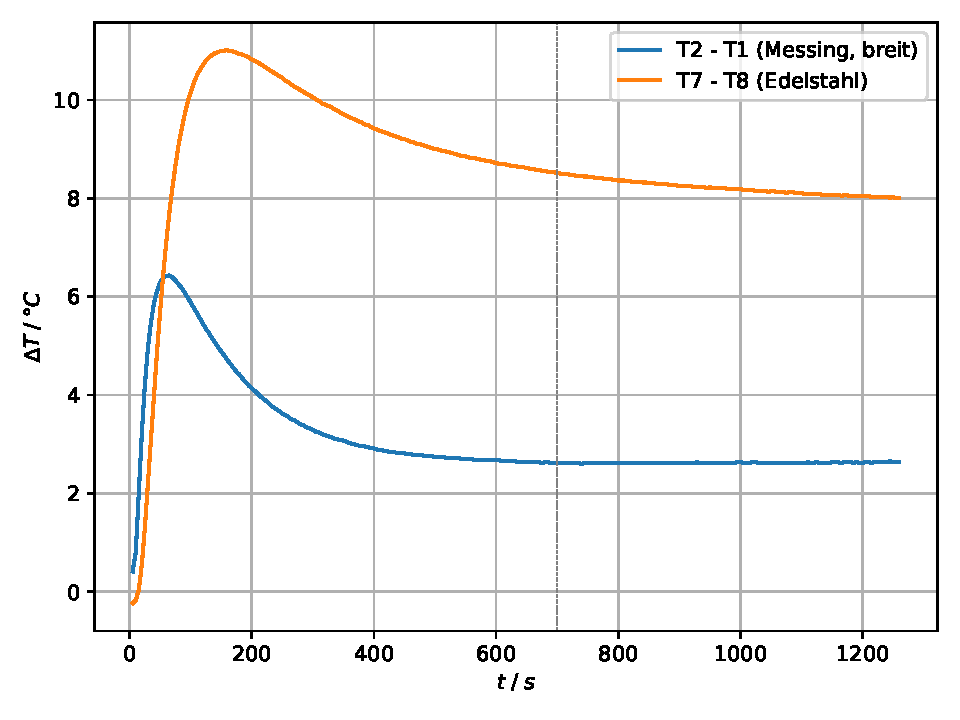
\includegraphics{build/plot_statisch_tdiff.pdf}
  \caption{Temperaturdifferenzen der nahen und fernen Thermoelemente für Messing (breit) und Edelstahl.}
  \label{fig:statisch_tdiff}
\end{figure}

Beim Vergleich der Temperaturdifferenzen der nahen und fernen Thermoelemente für Messing (breit) und Edelstahl in  \autoref{fig:statisch_tdiff} fällt auf,
dass die Temperaturdifferenz in Edelstahl nicht nur ein größeres Maximum annimmt,
sondern dieses außerdem zeitlich hinter dem von Messing liegt.

Die Erklärung für beide Beobachtungen ist,
dass Messing eine deutlich größere Wärmeleitfähigkeit als Edelstahl besitzt,
sodass die vom Peltierelement abgegebene Wärme schneller nach außen transportiert wird,
weshalb sich einerseits insgesamt kein so großer Temperaturunterschied ausbilden kann,
andererseits das ferne Thermoelement und damit die maximale Temperaturdifferenz früher erreicht wird.

Es lässt sich vermuten, dass die Maxima jeweils ungefähr den Zeitpunkt anzeigen,
an dem die vom Peltierelement ausgehende Wärmewelle das Ende des Stabs erreicht.
Weil die Wärme dann weniger gut nach außen abgeleitet werden kann,
nimmt die Temperatur am fernen Messpunkt schneller zu,
sodass die Temperaturdifferenz stagniert und schließlich wieder abnimmt.


\subsection{dynamische Methode}
\label{sec:auswertung_dynamisch}

\subsubsection{Messing (breit)}

In \autoref{fig:dynamisch_messing_breit} sind die Temperaturen am nahen und am fernen Thermoelement des breiten Messingstabs aufgetragen.
Es ist erkennbar, dass der ferne Temperaturverlauf kleinere Amplituden und eine Phasendifferenz aufweist.

\begin{figure}[H]
  \centering
  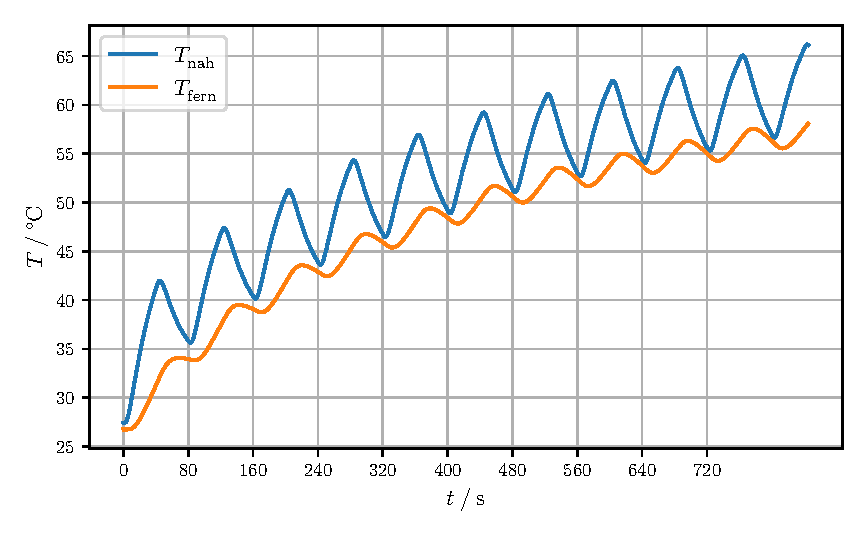
\includegraphics{build/plot_dynamisch_messing_breit.pdf}
  \caption{Zeitliche Entwicklung der Temperatur (nah/fern) des breiten Messingstabs.}
  \label{fig:dynamisch_messing_breit}
\end{figure}

In \autoref{tab:messing_breit} sind nun für jede Periode bis $t = \SI{800}{\second}$ die Amplituden, die Phasendifferenz und die nach \autoref{eqn:waermeleitfaehigkeit} berechnete Wärmeleitfähigkeit aufgelistet.
Zur Berechnung wurden $\rho$ und $c$ aus \autoref{tab:vorgegebeneDaten} übernommen.

\begin{table}[H]
     \centering
     \caption{Amplituden, Phasendifferenz und Wärmeleitfähigkeit für Messing (breit) für verschiedene Perioden.}
     \label{tab:messing_breit}
     \begin{tabular}{c c c c}
      \toprule
      $A_\text{nah} \mathbin{/} \si{\celsius}$ &
      $A_\text{fern} \mathbin{/} \si{\celsius}$ &
      $\symup{\Delta}t \mathbin{/} \si{\second}$ &
      $\kappa \mathbin{/} \si{\watt\per\meter\per\kelvin}$ \\
      \midrule
      \input{build/table_messing_breit.tex}
      \bottomrule
     \end{tabular}
\end{table}

Im Mittel ergibt sich $\kappa_\text{Messing, breit} = \SI{109.082 \pm 2.307}{\watt\per\meter\per\kelvin}$.
Die Frequenz der Wärmewelle berechnet sich nach \autoref{eqn:frequenz} direkt aus dem Kehrwert der Periodendauer,
mit der geheizt und gekühlt wird: $f = \SI{0.0125}{\per\second}$.
Die Wellenlänge berechnet sich nach Gleichungen \eqref{eqn:phasengeschwindigkeit} und \eqref{eqn:wellenlaenge} zu $\lambda = \SI{18.28 \pm 0.19}{\centi\meter}$.


\subsubsection{Aluminium}

Wie zuvor für den breiten Messingstab,
werden die nahen und fernen Temperaturverläufe für Aluminium geplottet,
und anschließend aus Amplitudenverhältnis, Phasendifferenz, und gegebenen $\rho$ und $c$
die Wärmeleitfähigkeit für jede Periode berechnet.

\begin{figure}[H]
  \centering
  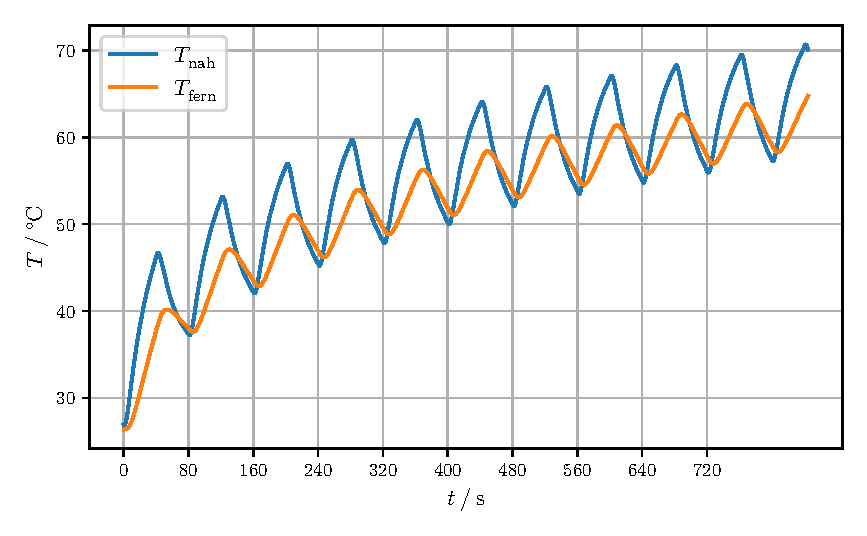
\includegraphics{build/plot_dynamisch_aluminium.pdf}
  \caption{Zeitliche Entwicklung der Temperatur (nah/fern) des Aluminiumstabs.}
  \label{fig:dynamisch_aluminium}
\end{figure}

\begin{table}[H]
     \centering
     \caption{Amplituden, Phasendifferenz und Wärmeleitfähigkeit für Aluminium für verschiedene Perioden.}
     \label{tab:aluminium}
     \begin{tabular}{c c c c}
      \toprule
      $A_\text{nah} \mathbin{/} \si{\celsius}$ &
      $A_\text{fern} \mathbin{/} \si{\celsius}$ &
      $\symup{\Delta}t \mathbin{/} \si{\second}$ &
      $\kappa \mathbin{/} \si{\watt\per\meter\per\kelvin}$ \\
      \midrule
      \input{build/table_aluminium.tex}
      \bottomrule
     \end{tabular}
\end{table}

Im Mittel ergibt sich $\kappa_\text{Aluminium} = \SI{248.228 \pm 5.176}{\watt\per\meter\per\kelvin}$.
Die Wellenlänge beträgt $\lambda = \SI{32.77 \pm 0.34}{\centi\meter}$,
die Frequenz ist wieder $f = \SI{0.0125}{\per\second}$.


\subsubsection{Edelstahl}

Zur Berechnung der Wärmeleitfähigkeit von Edelstahl werden die Messwerte des zweiten Durchlaufs mit
$\SI{200}{\second}$-periodischer Erhitzung verwendet.

\begin{figure}[H]
  \centering
  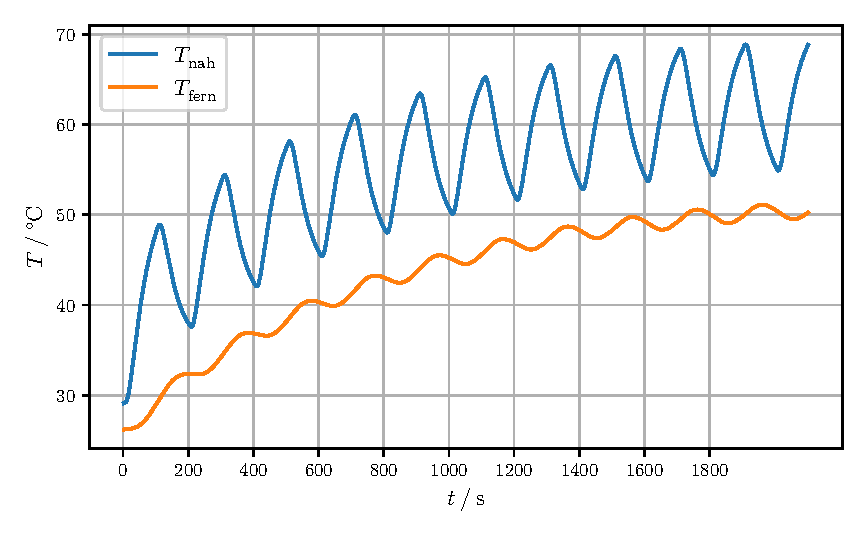
\includegraphics{build/plot_dynamisch_edelstahl.pdf}
  \caption{Zeitliche Entwicklung der Temperatur (nah/fern) des Edelstahlstabs.}
  \label{fig:dynamisch_edelstahl}
\end{figure}

\begin{table}[H]
     \centering
     \caption{Amplituden, Phasendifferenz und Wärmeleitfähigkeit für Edelstahl für verschiedene Perioden.}
     \label{tab:edelstahl}
     \begin{tabular}{c c c c}
      \toprule
      $A_\text{nah} \mathbin{/} \si{\celsius}$ &
      $A_\text{fern} \mathbin{/} \si{\celsius}$ &
      $\symup{\Delta}t \mathbin{/} \si{\second}$ &
      $\kappa \mathbin{/} \si{\watt\per\meter\per\kelvin}$ \\
      \midrule
      \input{build/table_edelstahl.tex}
      \bottomrule
     \end{tabular}
\end{table}

Im Mittel ergibt sich $\kappa_\text{Edelstahl} = \SI{15.109 \pm 0.199}{\watt\per\meter\per\kelvin}$.
Die Wellenlänge ist $\lambda = \SI{10.89 \pm 0.07}{\centi\meter}$.
Wegen der hier verwendeten Periodendauer von $\SI{200}{\second}$ ist die Frequenz der Wärmewelle $f = \SI{0.005}{\per\second}$.
